\documentclass[12pt]{article}                         
\pagestyle{plain} %-- Document Set Up Command

%-- Document Setup & Layout
\usepackage{fancyhdr}
\usepackage{comment}
\usepackage{multicol}
\usepackage[
  letterpaper,
  left=0.8in,
  right=0.8in,
  textheight=9.5in,
  bmargin=0.75in  % Adjust this value to push the footer down
]{geometry}

%-- Color & Text Formatting
\usepackage[svgnames]{xcolor} 
\usepackage{textcomp}
\usepackage{ulem}
\usepackage{graphicx}

%-- Math Packages
\usepackage{amsmath}     
\usepackage{amsfonts}
\usepackage{amstext}
\usepackage{amssymb}
\usepackage{latexsym}
\usepackage{bm}

%-- Graphics and Figures
\usepackage{graphicx}    
\usepackage{tikz}
\usepackage{pgfplots}
\usepackage{circledtext}
\usepackage{float}
\usepackage{caption}
\usepackage{subcaption}
\usetikzlibrary{decorations.markings, arrows.meta}
%-- Tables
\usepackage{array}      
\usepackage{tabularx}

%-- Lists
\usepackage{enumitem}    
%\usepackage{enumerate}
\usepackage{tasks}

%-- TikZ Libraries
\usetikzlibrary{shapes.geometric} 
\pgfplotsset{compat=1.18}
\tikzset{
    phase arrow/.style={
        postaction={decorate,
            decoration={
                markings,
                mark=at position 0.1 with {\arrow{Stealth}},
                mark=at position 0.3 with {\arrow{Stealth}},
                mark=at position 0.7 with {\arrow{Stealth}},
                mark=at position 0.9 with {\arrow{Stealth}}
            }
        }
    },
    phase arrow left/.style={
        postaction={decorate,
            decoration={
                markings,
                mark=at position 0.1 with {\arrow{Stealth[reversed]}},
                mark=at position 0.3 with {\arrow{Stealth[reversed]}},
                mark=at position 0.7 with {\arrow{Stealth[reversed]}},
                mark=at position 0.9 with {\arrow{Stealth[reversed]}}
            }
        }
    }
}
%-- Header/Footer
\pagestyle{fancy}
\fancyhf{} % Clear all header and footer fields
\fancyhead[L]{Jack Lingbeck} % Left header with name
\fancyhead[R]{February 10th, 2026} % Right header with date
\renewcommand{\headrulewidth}{0.4pt} % Horizontal line below the header
\rfoot{Page \thepage}
\lfoot{Homework 2}

\begin{document}
\large
\begin{center}
\fbox{\begin{tabular}{c}
\bf Math 675 Spring 2026: \\
\bf Homework 2 \\
\bf Due Tuesday, February 10th, 2026\\
\end{tabular}}
\end{center}

\section*{Question 1:}
Consider the uncoupled system: $$x'=3x, y'=-y$$
\begin{enumerate}
    \item[a)] Solve the system explicitly for general initial conditions $(x(0),y(0))=(x_0,y_0)$.
    \begin{flalign*}
    \quad x'(t) &= 3x   & \quad y'(t) &= -y &\\
    \quad \frac{dx}{dt} &= 3x &  \quad \frac{dy}{dt} &= -y \\
    \quad \int \frac{1}{x} dx &= \int 3 dt & \quad \int \frac{1}{y} dy &= \int -1 dt \\
    \quad \ln|x| &= 3t + c_1 & \quad \ln|y| &= -t + c_2 \\
    \quad e^{\ln|x|} &= e^{3t + c_1} & \quad e^{\ln|y|} &= e^{-t + c_2} \\
    \quad x &= e^{3t} e^{c_1} & \quad y &= e^{-t} e^{c_2} \\
    \text{Solution: } x(t) &= c_1 e^{3t} & \text{Solution: } y(t) &= c_2 e^{-t} & \\
    \text{IC: } x(0) = x_0 & = c_1 & \text{IC: } y(0) = y_0 & = c_2 \\
    \text{Final Solution: } x(t) &= x_0 e^{3t} & \text{Final Solution: } y(t) &= y_0 e^{-t} & \\
    \end{flalign*}
    \item[b)] Identify all equilibrium points of the system. \\
    $\left\{\begin{alignedat}{3} 3x  &&{}={} 0 \\ -y &&{}={} 0\end{alignedat}\right.
	\rightarrow
    \left\{\begin{alignedat}{3} x && = 0 \\ y && = 0\end{alignedat}\right.
	$ \\
    So like before, the only equilibrium point is at the origin $(0,0)$.
    \vspace{10cm}
    \item[c)] Using your explicit solution, determine the behavior of solutions as $t\to+\infty$:  
    Given out solutions from before: $x(t) = x_0 e^{3t}$ and $y(t) = y_0 e^{-t}$
    \begin{enumerate}
        \item[i)] initial conditions on the x-axis \\
        Using just $x=x_0 e^{3t}$, As $t\to +\infty$, \\
        If $x_0 > 0$ then $x(t) \to +\infty$ and if $x_0 < 0$ $x(t) \to -\infty$. \\\\
        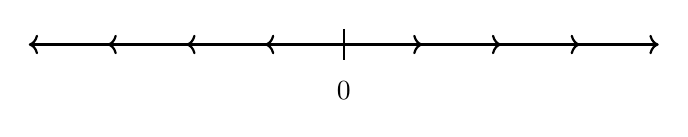
\begin{tikzpicture}
            \draw[thick, <->] (-4,0) -- (4,0);
            
            \draw[thick] (0,0.2) -- (0,-0.2) node[below=4pt] {0};
            
            \draw[thick, ->] (0.5,0) -- (1,0);
            \draw[thick, ->] (1,0) -- (2,0);
            \draw[thick, ->] (2,0) -- (3,0);
            
            \draw[thick, ->] (-0.5,0) -- (-1,0);
            \draw[thick, ->] (-1,0) -- (-2,0);
            \draw[thick, ->] (-2,0) -- (-3,0);
        \end{tikzpicture}

        \item[ii)] initial conditions on the y-axis \\
        Using just $y=y_0 e^{-t}$, As $t\to +\infty$, \\
        If $y_0 > 0$ then $y(t) \to 0$ and if $y_0 < 0$ $y(t) \to 0$. \\\\
        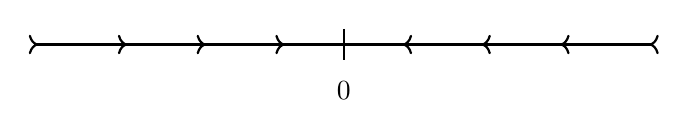
\begin{tikzpicture}
            \draw[thick, >-<] (-4,0) -- (4,0);
            
            \draw[thick] (0,0.2) -- (0,-0.2) node[below=4pt] {0};
            
            \draw[thick, <-] (0.75,0) -- (1,0);
            \draw[thick, <-] (1.75,0) -- (2,0);
            \draw[thick, <-] (2.75,0) -- (3,0);
            
            \draw[thick, <-] (-0.75,0) -- (-1,0);
            \draw[thick, <-] (-1.75,0) -- (-2,0);
            \draw[thick, <-] (-2.75,0) -- (-3,0);
        \end{tikzpicture}

        \item[iii)] initial conditions not lying on either axis \\
        \begin{minipage}{0.5\textwidth}
        
        \begin{itemize}
            \item If $t\to +\infty$ then solutions \\ approach the positive x-axis \\\\
            \item If $t\to -\infty$ then solutions \\ approach the negative x-axis
        \end{itemize}
        \end{minipage}
        \hfill
        \begin{minipage}{0.5\textwidth}
        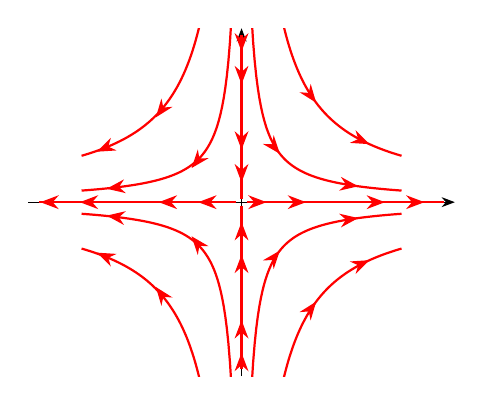
\begin{tikzpicture}
        \begin{axis}[
            width=7cm,
            height=6cm,
            axis lines = middle,
            samples=100,
            ymin=-5, ymax=5,
            xmin=-4, xmax=4,
            restrict y to domain=-10:10,
            xtick=\empty, ytick=\empty,
            axis line style={-Stealth}
        ]
            % Right Side (Pointing Right)
            \addplot[red, thick, phase arrow, domain=0.1:3] {1/x};
            \addplot[red, thick, phase arrow, domain=0.1:3] {4/x};
            \addplot[red, thick, phase arrow, domain=0.1:3] {-1/x};
            \addplot[red, thick, phase arrow, domain=0.1:3] {-4/x};

            % Left Side (Pointing Left)
            \addplot[red, thick, phase arrow left, domain=-3:-0.1] {1/x};
            \addplot[red, thick, phase arrow left, domain=-3:-0.1] {4/x};
            \addplot[red, thick, phase arrow left, domain=-3:-0.1] {-1/x};
            \addplot[red, thick, phase arrow left, domain=-3:-0.1] {-4/x};
            
            % Axis arrows
            \draw[red, thick, phase arrow ] (0.1, 0) -- (3.8, 0);     % Right
            \draw[red, thick, phase arrow left] (-3.8, 0) -- (-0.1, 0); % Left
            \draw[red, thick, phase arrow ] (0, 4.8) -- (0, 0.1);  % Down to origin
            \draw[red, thick, phase arrow ] (0, -4.8) -- (0, -0.1); % Up to origin
        \end{axis}
        \end{tikzpicture}
        \end{minipage} \\
    \item[d)] We can see from the behavior of the solutions as $t\to +\infty$ and $t\to -\infty$
    that the equilibrium point at the origin is a saddle point. This is because along the x-axis,
    the solutions diverge away from the origin, while along the y-axis, the solutions converge towards the origin. \\\\
    We can also see this as we take limits to positive and negitive \\ infinity of $x(t)=x_0 e^{3t}$ and $y(t)=y_0 e^{-t}$
    similar to what we have above, \\\\ 
    As $t\to +\infty$, $x(t) \to +\infty$ and $y(t) \to 0$, \\\\ 
    As $t\to -\infty$, $x(t) \to -\infty$ and $y(t) \to 0$. \\\\
    Because the limits for $y(t)$ are both $0$ yet the sign of infinity changes for $x(t)$, this tells us that this equilibrium point is a saddle point
    \vspace{5cm}
    \item[e)] Now we want to use Mathematica to plot the full phase portrait of this system. 
        \begin{figure}[H]
        \centering
        \includegraphics[width=0.4\textwidth]{Homework_2_Images/HW_2_Q1e.pdf}
        \end{figure}
        \end{enumerate}
\end{enumerate}

\section*{Question 2:}
Consider the uncoupled system: $$x'=-5x, y'=-y$$
\begin{enumerate}
    \item[a)] Solve the system explicitly for general initial conditions $(x(0),y(0))=(x_0,y_0)$ \\
    \begin{flalign*}
    \quad x'(t) &= -5x   & \quad y'(t) &= -y &\\
    \quad \frac{dx}{dt} &= -5x &  \quad \frac{dy}{dt} &= -y \\
    \quad \int \frac{1}{x} dx &= \int -5 dt & \quad \int \frac{1}{y} dy &= \int -1 dt \\
    \quad \ln|x| &= -5t + c_1 & \quad \ln|y| &= -t + c_2 \\
    \quad e^{\ln|x|} &= e^{-5t + c_1} & \quad e^{\ln|y|} &= e^{-t + c_2} \\
    \quad x &= e^{-5t} e^{c_1} & \quad y &= e^{-t} e^{c_2} \\
    \text{Solution: } x(t) &= c_1 e^{-5t} & \text{Solution: } y(t) &= c_2 e^{-t} & \\
    \text{IC: } x(0) = x_0 & = c_1 & \text{IC: } y(0) = y_0 & = c_2 \\
    \text{Final Solution: } x(t) &= x_0 e^{-5t} & \text{Final Solution: } y(t) &= y_0 e^{-t} & \\
    \end{flalign*}
    \vspace{5cm}
    
    \item[b)] Determine which variable decays faster as $t \to +\infty$, and justify your answer using the explicit solutions.
    
    As $t \to +\infty$, we can see both solutions $x(t) = x_0 e^{-5t}$ and $y(t) = y_0 e^{-t}$ 
    approach zero. However, the solution for $x(t)$ will decay faster than $y(t)$ 
    because $x(t)$ has a larger negative exponent compared to $y(t) = y_0 e^{-t}$, 
    which means that $x(t)$ will approach zero faster than $y(t)$ as time increases. \\

    \item[c)] Show that for any solution with $x_0 \neq 0$
    $$ \lim_{t \to +\infty} \frac{y(t)}{x(t)} = \infty $$
    Given our solutions $x(t) = x_0 e^{-5t}$ and $y(t) = y_0 e^{-t}$, we can compute the limit:
    $$\lim_{t \to +\infty} \frac{y(t)}{x(t)} = \lim_{t \to +\infty} \frac{y_0 e^{-t}}{x_0 e^{-5t}} = \lim_{t \to +\infty} \frac{y_0}{x_0} e^{4t}$$
    Since $e^{4t}$ increases to infinity as $t \to +\infty$, then the whole limit
    will also approach infinity. The only condition we need is that $x_0 \neq 0$ to ensure 
    that the denominator does not equal zero, which would make the limit undefined.
    \\\\
    \item[d)] Conclude that, except for the trajectory along the x-axis, 
    all other solution curves asymtotically converge to the x-axis as $t \to +\infty$.
    $$\lim_{t \to +\infty} x_0e^{-5t} = 0 \hspace{3cm} \lim_{t \to +\infty} y_0e^{-t} = 0$$
    Since we see that both solutions converge to 0, this implies that the slopes also converge 
    to horizontal lines, thus they become parrellel to the x-axis.
    \\\\
    \item[e)] Conclude that, except for the trajectory along the x-axis, 
    all other solution curves asymtotically converge to the y-axis as $t \to -\infty$.
    $$\lim_{t \to -\infty} x_0e^{-5t} = \infty \hspace{3cm}  \lim_{t \to -\infty} y_0e^{-t} = \infty$$
    Since we see that both solutions converge to $\infty$, this implies that the slopes also converge 
    to vertical lines, thus they become parrellel to the y-axis.

\end{enumerate}

\vspace{6cm}

\section*{Question 3:}
Show that for a linear, homogeneous system of ODE with $a,b,c,d \neq 0$, where \\ 
$x'$ and $y'$ are not scalar multiples of each other, the only equilibrium point is $(0,0)$.
$$x' = ax + by, \hspace{1cm} y' = cx + dy$$
First, lets find the determinate of this system, since we are basically talking about linear independence.
Let a matrix A, be the coeffient matrix of this system. \\ 
We want then force $\det(A) \neq 0$ so $x'$ and $y'$  are not scalar multiples of each other
\begin{equation}
    A = \begin{vmatrix} a & b \\ c & d \end{vmatrix} = ad - bc \neq 0
\end{equation}
Now, let's try to find the equilibrium points of this system.
We set $x' = 0$ and $y' = 0$ and solve for $x$ and $y$ . \\
$$\left\{\begin{alignedat}{3} ax &+ by &&{}={} 0 \\ cx &+ dy &&{}={} 0\end{alignedat}\right.
\rightarrow
\left\{\begin{alignedat}{3} ax &+ &&{}={} -by \\ cx &+ dy &&{}={} 0\end{alignedat}\right.
\rightarrow
\left\{\begin{alignedat}{3} x &+ &&{}={} -\frac{by}{a} \\ cx &+ dy &&{}={} 0\end{alignedat}\right.
$$ \\
Now lets substitute the first equation into the second equation to solve for $y$.
\begin{equation}
0 = cx+dy = c\left(-\frac{by}{a}\right) + dy = -\left(\frac{bc}{a}\right)y + dy = y\left(d - \frac{bc}{a}\right)
\end{equation}
This is where things get interesting, since we're given $a,b,c,d \neq 0$ and $ad - bc \neq 0$, 
then we can see we have two solutions for this equation $y = 0$ or $d - \frac{bc}{a} = 0$.
\[0 = d-\frac{bc}{a} \implies ad-bc = 0\]
But we are given that $ad - bc \neq 0$ from equation $(1)$, so the only valid solution for equation $(2)$ 
is $y = 0$. Now we can substitute this back to solve for $x$.
$$x = -\frac{by}{a} = -\frac{b \cdot 0}{a} = 0$$
Therefore, the only equilibrium point is $(0,0)$.

\vspace{5cm}
\section*{Question 4:} 
Consider the coupled ODE system $$x' = -y, \hspace{1cm} y' = -x$$
\begin{enumerate}
    \item[a)] Use Mathematica to plot the phase portrait of this system. 
        \begin{figure}[H]
        \centering
        \includegraphics[width=0.4\textwidth]{Homework_2_Images/HW_2_Q4a.pdf}
        % StreamPlot[{-y, -x}, {x, -3, 3}, {y, -3, 3}, 
        % StreamColorFunction -> None, 
        % StreamPoints -> {{{{1, 0}, Red}, {{-1, -1}, Green}, {{-1, 2}, Orange}, Automatic}}]
        \end{figure}
     \item[b)] Follow the outline below to prove that the trajectories of the system are hyperbolas 
                of the form $x^2 - y^2 = C$ where $C$ is a constant.
    \item[i)] Show that the system of ODEs implies $x\frac{dx}{dt} - y\frac{dy}{dt} = 0$.
    $$x' = -y, \hspace{1cm} y' = -x$$
    $$\frac{x'}{y} = -1 \hspace{1cm} \frac{y'}{x} = -1$$
    $$\frac{x'}{y} = \frac{y'}{x}$$
    $$xx' = yy'$$
    $$x\frac{dx}{dt} - y\frac{dy}{dt} = 0$$

    \item[ii)] Use the chain rule to show that $\frac{1}{2}\frac{d}{dt}(x^2) = x\frac{dx}{dt}$.
    $$\frac{1}{2}\frac{d}{dt}(x(t))^2 = \frac{1}{2}(2)x(t)\frac{dx}{dt} = x(t)\frac{dx}{dt}$$

    \vspace{2cm}
    \item[iii)] Substitute the identity for both variables in part ii) into EQ(1)
    $$x\frac{dx}{dt} - y\frac{dy}{dt} = 0$$
    $$\frac{1}{2}\frac{d}{dt}(x^2) - \frac{1}{2}\frac{d}{dt}(y^2) = 0$$
    \item[iv)] Integrate both sides of the equation and use the fundamental theorem of calculus to get the results
    $$\frac{d}{dt}\left(\frac{x^2}{2} - \frac{y^2}{2}\right) = 0$$
    $$\int \frac{d}{dt}\left(\frac{x^2}{2} - \frac{y^2}{2}\right) dt = \int 0 dt$$
    $$\frac{x^2}{2} - \frac{y^2}{2} = C$$
    $$x^2 - y^2 = C$$
\end{enumerate}

\section*{Question 5:} 
In this problem we consider the same coupled ODE system as in the previous problem $$x'= -y, y'=-x$$
We want to decouple and solve this analytically. So please do the following:
\begin{enumerate}
    \item[a)] Introduce new variables $u$ and $v$ defined by $u = x + y$ and $v = x - y$. \\ Solve for the variables $u,v$ in terms of $x$ and $y$.
    $$u + v = (x+y) + (x-y) \hspace{1cm} u - v = (x+y) - (x-y)$$
    $$u + v = 2x \hspace{1cm} u - v = 2y$$
    $$\frac{u + v}{2} = x \hspace{1cm} \frac{u - v}{2} = y$$
    
    \item[b)] Rewrite the ODE system in terms of $u$ and $v$ using the previous part
    We want to differentiate $u$ and $v$ with respect to $t$ to get $u'$ and $v'$. 
    Then substitute the original ODEs for $x'$ and $y'$ to get the new ODEs in terms of $u$ and $v$.
    $$u' = x' + y' = -y - x = -(x+y) = -u$$
    $$v' = x' - y' = -y + x = (x-y) = v$$

    \item[c)] Solve for $u(t) $ and $v(t)$ starting from an arbirary initial condition $(u_0, v_0)$.
    \begin{flalign*}
    \quad u'(t) &= -u   & \quad v'(t) &= -v &\\
    \quad \frac{du}{dt} &= -u &  \quad \frac{dv}{dt} &= v \\
    \quad \int \frac{1}{u} du &= \int -1 dt & \quad \int \frac{1}{v} dv &= \int 1 dt \\
    \quad \ln|u| &= -t + c_1 & \quad \ln|v| &= t + c_2 \\
    \quad e^{\ln|u|} &= e^{-t + c_1} & \quad e^{\ln|v|} &= e^{t + c_2} \\
    \quad u &= e^{-t} e^{c_1} & \quad v &= e^{t} e^{c_2} \\
    \text{Solution: } u(t) &= c_1 e^{-t} & \text{Solution: } v(t) &= c_2 e^{t} & \\
    \text{IC: } u(0) = u_0 & = c_1 & \text{IC: } v(0) = v_0 & = c_2 \\
    \text{Final Solution: } u(t) &= u_0 e^{-t} & \text{Final Solution: } v(t) &= v_0 e^{t} & \\
    \end{flalign*} 

    \item[d)] Finally, using the answer above, write the general solution in terms of $x(t)$ and $y(t)$.
    Make sure to also write starting from the initial conditions $(x_0, y_0)$.
    We can note that if $t=0$ implies $u(0)=u_0$ and $v(0)=v_0$ then we can also conclude
    that we can obtain the initial conditions of $u$ and $v$ in terms of the initial conditions of $x$ and $y$.
    \[u(0) = x(0) + y(0) = x_0 + y_0 \quad\quad\quad\quad  v(0) = x(0) - y(0) = x_0 - y_0\]
    Now, substitute these modified initial conditions into our solutions to get:
    \begin{equation*}
    \begin{aligned}
        x(t) &= \frac{1}{2}\left[u(t) + v(t)\right] \\
            &= \frac{1}{2}\left[u_0 e^{-t} + v_0 e^{t}\right] \\
            &= \frac{1}{2}\left[(x_0 + y_0) e^{-t} + (x_0 - y_0) e^{t}\right] \\
            &= \frac{1}{2}\left[x_0(e^{-t} + e^{t}) + y_0(e^{-t} - e^{t})\right] \\
            &= x_0 \cosh(t) - y_0 \sinh(t)
    \end{aligned}
    \qquad \qquad % Adds space between columns
    \begin{aligned}
        y(t) &= \frac{1}{2}\left[u(t) - v(t)\right] \\
            &= \frac{1}{2}\left[u_0 e^{-t} - v_0 e^{t}\right] \\
            &= \frac{1}{2}\left[(x_0 + y_0) e^{-t} - (x_0 - y_0) e^{t}\right] \\
            &= \frac{1}{2}\left[x_0(e^{-t} - e^{t}) + y_0(e^{-t} + e^{t})\right] \\
            &= -x_0 \sinh(t) + y_0 \cosh(t)
    \end{aligned}
    \end{equation*}
\end{enumerate}

\end{document}